\chapter{Introduction}
\label{ch:into} % This how you label a chapter and the key (e.g., ch:into) will be used to refer this chapter ``Introduction'' later in the report. 
% the key ``ch:into'' can be used with command \ref{ch:intor} to refere this Chapter.

\textbf 

Instability is defined as the real proportion of profit dispersion for a specific security or market. Contributing to and benefitting from the market has never been easy due to its evident weakness and severe unpredictability, in which shares and values might increase or fall dramatically. Typically, the more risky the security, the greater the degree of uncertainty. The fluctuation of basic stocks' true costs is known as documented instability or "known unpredictability." They have shown to be the most difficult yet rewarding and beneficial for business. There are several evaluations of market behavior.

Time series forecasting is a significant area of forecasting in which previous observations of the same variable are gathered and evaluated to create a model that describes the underlying relationship. The model is then used to extrapolate the time series forward. The autoregressive integrated moving average (ARIMA) model is a popular and well-known time series model. The ARIMA model's popularity stems from its statistical features as well as the well-known Box-Jenkins approach \citep{DEGROOT1991177} used in model development. However, the assumption of linear data renders them unsuitable for nonlinear time series modeling.

Unlike sequence-aligned models \citep{wu2020deep}, the transformer analyzes a full series of data and uses self-attention mechanisms to learn information from the sequence, allowing us to model variable relationships without regard for their distance in the input sequences. In particular, because the attention mechanism may not only gather global information but also focus on relevant material, it has the potential to ease the curse of dimensionality significantly.


We use the Y-finance dataset to forecast a single ticker, taking into account several factors 
such as volume, high, close, and open. Utilizing nine tickers, we are able to achieve 
prediction characteristics whereby the tenth ticker is anticipated by utilizing all nine ticker 
values. To achieve these kinds of significant modifications, we approximate a method wherein 
the model's prediction weights produce the particular shift in testing and prediction values. 
Ultimately, based on the kind of algorithm selected and developed, a general comparison 
analysis using various time instances is confirmed. 

%%%%%%%%%%%%%%%%%%%%%%%%%%%%%%%%%%%%%%%%%%%%%%%%%%%%%%%%%%%%%%%%%%%%%%%%%%%%%%%%%%%
\section{Background}
\label{sec:into_back}


\textbf
Stockbrokers, traders, and investors that purchase, sell, or share transactions 
collectively make up the stock market. Because so many businesses post their stock lists 
online, investors find their stocks appealing \citep{bhattacharjee2019stock}. The size of the 
markets and the speed at which deals are completed now make it impractical for investors to use 
their own experience, which they once used to discern market trends. A nation's economic status 
affects a number of industries, including investment banking, metals, agriculture, and finance, 
either directly or indirectly. The fundamental law of supply and demand dictates that the 
growth of these industries depends on their volatility. Due to the fact that investors have 
been attempting various methods since the 17th century in order to increase the returns on their 
investments by learning about various firms \citep{mehta2021stock}. There is a noticeable 
increase in demand for stock market services. Accurately predicting future financial outcomes is the 
main goal of stock price prediction. Machine Learning algorithms have shown promise in a number 
of sectors in recent years, and as a result, many traders are using these strategies in their 
particular domains. 

An accounting forecast can be viewed as a difficult time-varying prediction. A transformer in 
deep learning is a model that uses the self-attention process and weights each incoming data 
component differently based on its significance. Transformers are intended to evaluate 
sequential input data, including plain language, much like recurrent neural networks (RNNs). 
But transformers handle the whole input all at once, unlike RNNs. The statistical prediction 
instruments that have been most widely used are ARIMA models. Though regrettably, not all 
future occurrences are predicted by this model with the same level of accuracy. This is 
because, following three or four predicted values, the forecasts converge to the series mean. 
Usually, the maximum likelihood model or the least squares estimation model are used to 
estimate the parameters of ARIMA models. In several disciplines, most notably economics, 
artificial neural networks (ANNs) have been utilized for prediction. 

%%%%%%%%%%%%%%%%%%%%%%%%%%%%%%%%%%%%%%%%%%%%%%%%%%%%%%%%%%%%%%%%%%%%%%%%%%%%%%%%%%%
\section{Problem statement}
\label{sec:intro_prob_art}
Given the available computing power and training constraints, is it possible to build and train 
both a transformer neural networks and an ARIMA-ANN hybrid model using historical stock price 
data? What distinguishes Transformer Neural Networks' stock price prediction skills from those 
of the ARIMA-ANN hybrid model, and what are their distinctive characteristics and performance 
metrics? What insights can be acquired on the capacity of these models to adjust to shifting 
market conditions, and how does the selection of prediction model affect the process of making 
investments over a certain time period?

%%%%%%%%%%%%%%%%%%%%%%%%%%%%%%%%%%%%%%%%%%%%%%%%%%%%%%%%%%%%%%%%%%%%%%%%%%%%%%%%%%%
\section{Aims and objectives}
\label{sec:intro_aims_obj}


\textbf{Aims:} 
Taking into account the available processing capacity and training limitations, the purpose of this research is to examine whether it is feasible to construct and train Transformer Neural Networks and the ARIMA-ANN hybrid model using historical stock price data. The study attempts to identify the unique traits, performance measures, and stock price prediction abilities of these algorithms. The research also aims to learn more about the ability of Transformer Neural Networks and the ARIMA-ANN hybrid model to adjust to changing market conditions. The ultimate goal is to comprehend the ways in which the choice of prediction model affects the process of making investments over a given time frame.


\textbf{Objectives:} 
    \label{sec:first objective}
    \begin{enumerate}
        \item With regard to training limitations and available processing capacity, assess the feasibility of constructing and training Transformer Neural Networks as well as the ARIMA-ANN hybrid model using historical stock price data.
        \item Give a detailed explanation of the unique characteristics of the ARIMA-ANN hybrid model and Transformer Neural Networks to offer a more sophisticated grasp of their strengths and weaknesses.
        \item Consider certain performance metrics, accuracy, and dependability when choosing a prediction model (ARIMA-ANN hybrid or Transformer Neural Networks), and analyze the impact on the investment decision-making process.
    \end{enumerate}





%%%%%%%%%%%%%%%%%%%%%%%%%%%%%%%%%%%%%%%%%%%%%%%%%%%%%%%%%%%%%%%%%%%%%%%%%%%%%%%%%%%
\section{Solution approach}
\label{sec:intro_sol} % label of Org section
As financial data and analysis continue to progress, we are using Yahoo finance data more and more to create a system that displays the broad changes observed in the data projected for stocks. With ten different labels representing the stocks of the businesses, the proposed work intends to construct a TNN-based prediction system that displays the entire design on stock tickers. Nine tickers in total are utilized to illustrate the general viewpoint of feature extractions on those tickers through the usage of the characteristics of high, low, close, open, adj-close, and volume. With the help of the several features mentioned above and a multi-objective function with a linear and non-linear structure, one of the ticker's expected values is determined. Visual representation of the overall changes in the design is demonstrated by comparing the predicted values with the original condition.
Taking into consideration the different open, close, volume, and high elements, we produce a forecast for a particular ticker using the Y-finance dataset. In order to implement the prediction features, we use nine tickers, with the tenth ticker being predicted based on the values of the nine tickers. To achieve these effective adjustments, we compute a fix whose prediction weights on the model yield the specific shift in testing and prediction outcomes. Finally, an overall analysis of comparisons across different time periods

%%%%%%%%%%%%%%%%%%%%%%%%%%%%%%%%%%%%%%%%%%%%%%%%%%%%%%%%%%%%%%%%%%%%%%%%%%%%%%%%%%%
\section{Dataset} %  use this section 
\label{sec:intro_sum_results} % label of summary of results
We get stock prices from Yahoo! Finance using Python modules and a custom method. We collect the open, close, adj close, high, low, prices, and volume of ten different firms once every one day, one hour, and five minutes. We have three years of data at one-day intervals, one year at one-hour intervals, and the last 60 days at five-minute intervals. The prices are standardized by a min-max scaler. 95\% of the stock data is used to train the models, with the remaining 5\% for validation and testing. We expect the algorithms to finally build a market pattern based on the prices of ten corporations during the last three years. The program will be trained on data from nine different organizations before being used to forecast data from a tenth.

\begin{figure}[ht]
    \centering
    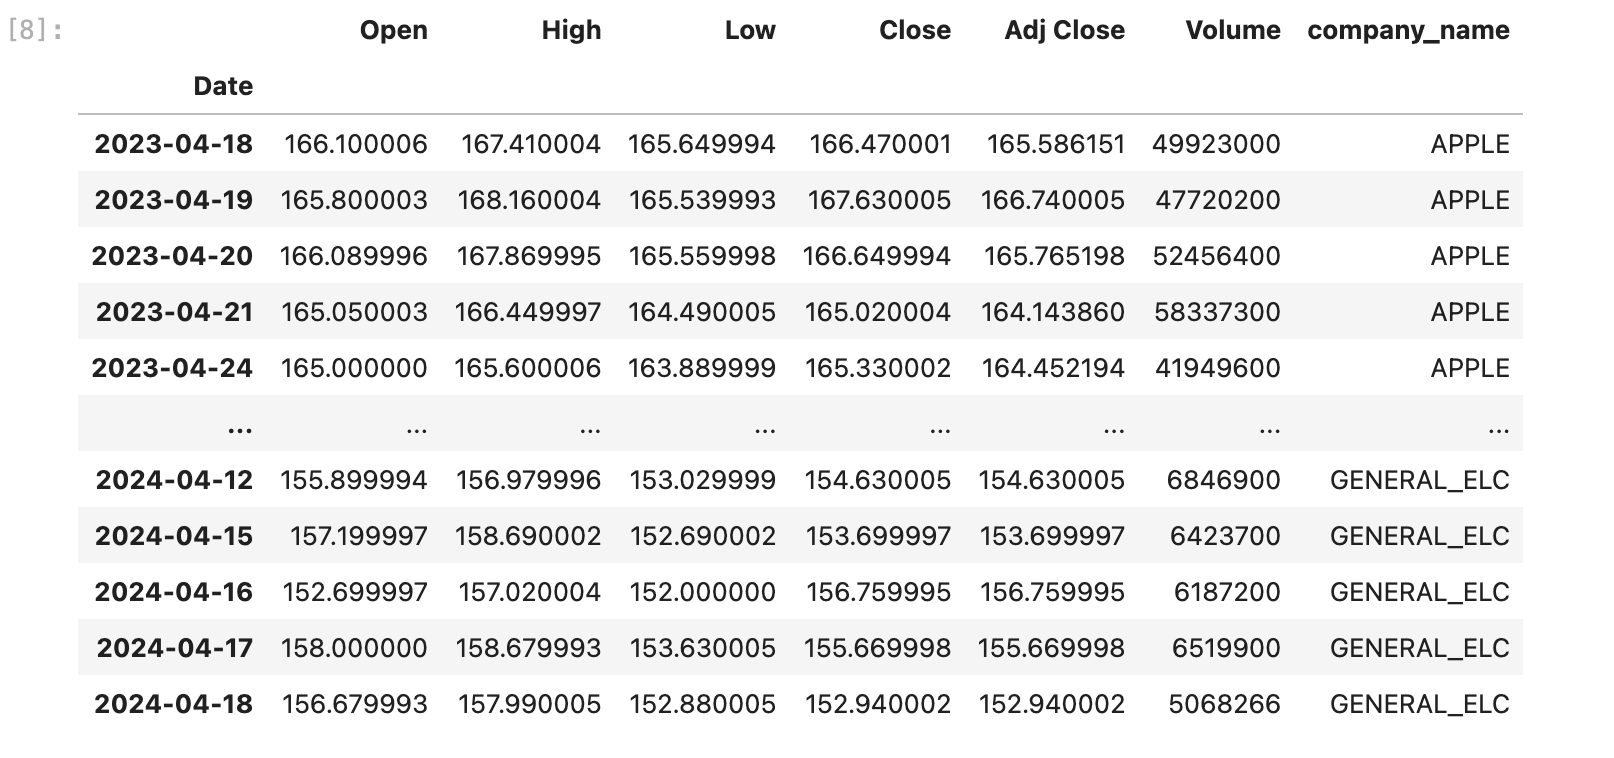
\includegraphics[scale=0.3]{figures/Dataset.png}
    \caption{Representing the dataset with time period as 1hr.}
    \label{fig:chart_a}
\end{figure}





%%%%%%%%%%%%%%%%%%%%%%%%%%%%%%%%%%%%%%%%%%%%%%%%%%%%%%%%%%%%%%%%%%%%%%%%%%%%%%%%%%%
%%%%%%%%%%%%%%%%%%%%%%%%%%%%%%%%%%%%%%%%%%%%%%%%%%%%%%%%%%%%%%%%%%%%%%%%%%%%%%%%%%%
\section{Summary of contributions and achievements} %  use this section 
\label{sec:intro_sum_results} % label of summary of results



%%%%%%%%%%%%%%%%%%%%%%%%%%%%%%%%%%%%%%%%%%%%%%%%%%%%%%%%%%%%%%%%%%%%%%%%%%%%%%%%%%%

